\documentclass[11pt]{article} 
\def\name{Hunter Kruger-Ilingworth}
\def\doctitle{Capstone Project Report}
\def\subjectcode{MA3832}
\def\studentnumber{14198489}
% Geometry and Layout
    \usepackage[margin=0.75in]{geometry}
    \usepackage{parskip}
    \usepackage{placeins} % FloatBarrier

% Graphics and Diagrams
    \usepackage{wrapfig}

    \usepackage{xcolor}
    \usepackage{graphicx} % Required for inserting images
    \usepackage[american]{circuitikz}
    \usepackage{tikz}
    \usepackage{tikz-3dplot}
    \usetikzlibrary{arrows.meta}
    \usetikzlibrary{positioning}  % Add this line to load the positioning library
    \usepackage{pgfplots}
    \pgfplotsset{compat=newest}
    \usepackage{listings}
    \usepackage{tcolorbox}

% CSV Table input
    \usepackage[table]{xcolor}
    \usepackage{csvsimple, booktabs}

% Code Chunk Formatting
    \definecolor{comment_color}{rgb}{0.52,0.38,0.78}
    \definecolor{keyword_color}{rgb}{0.84,0.27,0.3}
    \definecolor{background_color}{rgb}{0.95,0.95,0.95}
    \usepackage{inconsolata} % Consolas-style font from the inconsolata package

\lstset{
    backgroundcolor=\color{background_color},   % Choose the background color
    commentstyle=\color{comment_color},       % Style of comments
    keywordstyle=\color{keyword_color},        % Style of keywords
    stringstyle=\color{red},              % Style of strings, assuming red
    basicstyle=\tiny\ttfamily, % Set font size, monospaced font, and color        
    breakatwhitespace=false,              % Automatic line breaking only at whitespace
    breaklines=true,                      % Automatic line breaking
    captionpos=t,                         % Caption position is on top
    keepspaces=true,                      % Keeps spaces in text
    numbers=left,                         % Line number position
    numbersep=5pt,                        % How far the line numbers are from the code
    showspaces=false,                     % Show spaces in the code
    showstringspaces=false,               % Underline spaces within strings only
    showtabs=true,                       % Show tabs within strings adding particular underscores
    % framexleftmargin=5pt,                       % Extra space on the left for better aesthetics
    xleftmargin=0.05\textwidth,                 % Indent from the left
    xrightmargin=0.05\textwidth,                % Indent from the right
    tabsize=1,                            % Sets default tab size
    title=\lstname                        % Show the filename of files included with \lstinputlisting
}
% Text Content / Math
    \usepackage{lipsum} % Dummy text
    \usepackage{hyperref}
    \usepackage{amsmath} % For sum symbol and other math formatting
    \usepackage{amssymb}

% Headers and Footers
    \usepackage{lastpage}
    \usepackage{fancyhdr}
    \makeatletter
    \renewcommand{\@seccntformat}[1]{}
    \makeatother
    \pagestyle{fancy}
    \fancyhf{} 
    \setlength{\headheight}{15pt}
    \fancyhead[L]{\subjectcode{} - \doctitle{}}
    \fancyhead[R]{} % Rearrange as you please
    \fancyfoot[L]{\name{}}
    \fancyfoot[R]{Page \thepage\ of \pageref{LastPage}} 
    \renewcommand{\headrulewidth}{0pt}

% Caption and Referencing Customization
    \usepackage[justification=centering]{caption}
    \usepackage{cleveref}
    \usepackage{nameref}
    \DeclareCaptionLabelSeparator{IEEE}{.\quad }
    \captionsetup[figure]{name=Fig., labelsep=IEEE}
    \captionsetup{format=hang, labelfont=bf}
    \captionsetup{justification=raggedright,singlelinecheck=false}

% Document Metadata and First Page Formatting
    \title{\doctitle{}\\\large{James Cook University Cairns}}
    \author{\name{} (\studentnumber{})}
    \date{\today}

% Referencing

    \usepackage[noadjust]{cite} % For IEEE-style citations
    \renewcommand{\refname}{} % Remove "References" title

% Editing quality of life
    \usepackage{todonotes} 

%Choose which files are re-rendered (saves rendering time)
%\includeonly{}

\newcommand{\insertimage}[3]{
\begin{figure}[h]
    \centering
    \includegraphics[height= 200px]{#1} % Image filename
    \centering 
    \caption{#2} % Caption
    \label{#3} % Label
\end{figure}
}

\newcommand{\insertimagesize}[4]{
\begin{figure}[h]
    \centering
    \includegraphics[height= #4]{#1} % Image filename
    \centering 
    \caption{#2} % Caption
    \label{#3} % Label
\end{figure}
}

\newcommand{\insertbigimage}[3]{
\begin{figure*}[h]
    \centering
    \includegraphics[width=\linewidth]{#1} % Image filename
    \caption{#2} 
    \label{#3} 
\end{figure*}
}

\newcommand{\codeblockfile}[4]{
    \lstinputlisting[language=#1, caption={#2}, label=#3]{#4}
}

\newcommand{\E}[1]{
    \cdot 10^{#1}
}

\newcommand{\abs}[1]{
    \left\lvert #1 \right\rvert
}

\newcommand{\note}[1]{\textcolor{red}{#1}} %create a note for yourself


\definecolor{codegray}{gray}{0.9} % Light gray color
\newcommand{\code}[1]{\colorbox{codegray}{\texttt{\detokenize{#1}}}} % Command for inline code

\begin{document}


    % Create the title page
    \begin{titlepage}
        \maketitle
        \thispagestyle{empty} %suppresses page numbering on the title page
    \end{titlepage}

    % Table of Contents
    \thispagestyle{empty} % Suppresses page numbering on the contents page
    \onecolumn
    \tableofcontents
    \listoffigures
    \listoftables
    \clearpage
    
    \section{Introduction }

"AI as a creative tool has improved leaps and bounds since its early incarnations. Generating still images that are interesting, sophisticated and photorealistic is now an easy process that can be done by anybody with an interest, some patience and determination" \cite{scott2024ethics}. The prevalence of AI among the general public has led to extensive dialogue about their ethical implications in producing artwork, or for manufacturing misinformation. One such example of the use of AI is tools like \textit{DALL-E} and \textit{Stable Diffusion}, which generate images from text prompts. In the current digital age, we cannot rely on the transparency of the source of an image, so there exists a need to be able to identify whether an image has been generated by an AI, or a real artist. \Cref{fig:ai_generated_images} shows some examples of AI generated images, which are becoming increasingly difficult to distinguish from real images as the technology improves, underscoring the need for reliable detection methods.

\begin{figure}[h]
    \centering
    
\includegraphics[width=0.8 \linewidth]{figures/ai_generated_images_from_seeing_is_not_believing.png} % Image filename
    \centering
    \caption{AI generated images \cite{lu2023seeingbelievingbenchmarkinghuman}} % Caption
    \label{fig:ai_generated_images} % Label
\end{figure}

\cite{lu2023seeingbelievingbenchmarkinghuman} evaluates both human and AI capabilities in detecting fake images, showing that humans are often deceived by advanced image generation models, while AI-based detection algorithms outperform humans but still misclassify 13\% of images. The study introduction of the Fake2M dataset and new benchmarks (HPBench and MPBench) aims to drive further research and improve the reliability of AI-generated content detection.

\cite{bird2023cifakeimageclassificationexplainable} presents a computer vision approach to distinguishing AI-generated images from real ones, utilising a synthetic dataset created with Latent Diffusion, classification via Convolutional Neural Networks, and interpretability through Grad-CAM. Achieving nearly 93\% accuracy, the study also introduces the CIFAKE dataset, a large collection of real and synthetic images, to support further research on the detection of AI-generated imagery.

It is therefore evident that past research has shown that it is possible to classify images as AI-generated or not, with a high degree of accuracy. This report will explore the process of training a neural network to classify images as either AI-generated or not, and then deploying this model to AWS SageMaker for inference, and evaluating it against comparable models. This is done so that people can distinguish between AI-generated and real images, ultimately as a tool to identify the spread of misinformation and other harms.
    \newpage

\section{Dataset}

The dataset used for this project was a competition dataset from Hugging Face, held in 2023 \cite{huggingface_competitions_aiornot}.
The dataset consists of 62,060 images, and is 2.37GB in size, being pre-split into training and tesing sets, as summarised in \cref{tab:dataset_summary,tab:class_counts}, where it can be seen that the testing set has the class labels withheld due to the competition setting, restricting this analysis to the 18,618 training images, which we can sub-divide and validate with known labels.
\begin{table*}[h]
    \centering
    \begin{minipage}{0.48\textwidth}
        \centering
        \begin{tabular}{ll}
            \toprule
            \textbf{Feature} & \textbf{Description} \\
            \midrule
            \code{id}     & Index filename \code{34.jpg} \\
            \code{image}  & The Image (512x512) \\
            \code{label}  & Binary class label \\
            \bottomrule
        \end{tabular}
        \caption{Dataset features and their descriptions.}
        \label{tab:dataset_summary}
    \end{minipage}\hfill
    \begin{minipage}{0.48\textwidth}
        \centering
        \begin{tabular}{lcc}
            \toprule
            \begin{tabular}[c]{@{}l@{}}\textbf{Class} \\ \textbf{Label}\end{tabular} & 
            \begin{tabular}[c]{@{}c@{}}\textbf{Train} \\ \textbf{Count}\end{tabular} & 
            \begin{tabular}[c]{@{}c@{}}\textbf{Test} \\ \textbf{Count}\end{tabular} \\
            \midrule
            AI (1)      & 10,330 $(55.5\%)$ & NA \\
            Not AI (0)  & 8,288 $(45.5\%)$ & NA \\
            \bottomrule
            \textbf{Total}       & 18,618 & 43,442 \\
        \end{tabular}
        \caption{Counts of each class label in the training and testing sets}
        \label{tab:class_counts}
    \end{minipage}
\end{table*}

\Cref{code:data_wrangling} shows the code used to load the dataset, and split it into training, validation, and test sets. It can be seen that the splitting method for the data was to 
- holdout 500 images for final testing (only 500 was chosen due to a bandwidth issue on the AWS endpoint, further elaborated on in \Cref{sec:model_deployment}),
- split the remaining training data into three sets, the small train, train and test set, being 10\%, 70\%, and 20\% of the remaining data respectively.
- to ensure class balance between these sets, random oversampling was employed. This was because \cref{tab:class_counts} shows that if a model were to guess AI all the time, it could get an accuracy of 55.5\%

\Cref{code:data_wrangling}, in the appendix shows the code used to load the dataset from HuggingFace. It can then be seen that the splitting sceme described above is done using hugging faces \code{train_test_split} method. The HuggingFace dataset object is converted to numpy arrays. Then \code{Imblearn}'s \code{RandomUnderSampler} is used to ensure class balance, as to not bias the majority class.



This data was converted to npz files, due to their efficient storage and loading capabilities. After conversion, the data was uploaded to an S3 bucket for easy access during model training and evaluation. Uploading to S3 buckets was critical, as it meant that there was no longer a reliance on the RAM allocation of the sagemaker notebook environment - it could be loaded in from the S3 bucket in batches, which has the benefit of being a more scalable solution.

\begin{figure}[h]
    \centering
    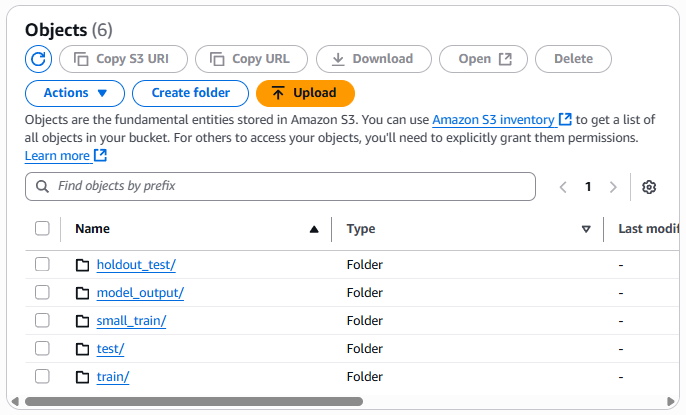
\includegraphics[width=250px]{figures/s3_bucket_screenshot.png} % Image filename
    \centering
    \caption{Screenshot of S3 Bucket with training data in AWS Console} % Caption
    \label{fig:s3_bucket} % Label
\end{figure}



    
\newpage

\section{Model Structure}

With the data acquired from HuggingFace, the process of making a machine learning model could begin. The model that was developed was a convolutional neural network (CNN). It accepts full-size images of shape $(512, 512, 3)$, with each image being an rgb image with values ranging from 0 to 255. \Cref{code:model_definition} shows the \code{src/model.py} file, which was called by the \code{main.ipynb} and \code{src/train.py} files to train and tune the model.

\begin{figure}[h]
    \lstinputlisting[language=Python, caption=Model definition code extract, label=code:model_definition]{code_chunks/sec_3_model.py}
\end{figure}

For the first section, a \code{Conv2D} layer was applied with a kernel size of $3{\times}3$ and a tunable number of filters, $f_{1}$. The stride was fixed at its default value of $1$, with padding set to \emph{same} which preserves the spatial dimensions of the input feature maps, at the cost of increased computational cost. A \code{ReLU} activation function was used due to its simplicity and its ability to address vanishing gradients.

This was followed by a pooling layer, where either max pooling or average pooling could be selected. By default, the pooling operation uses a window of size $2{\times}2$ with stride $2$, reducing the spatial resolution of the feature maps by half while retaining the most salient information.

The second convolutional block repeated this process with a kernel size of $3{\times}3$ and a tunable number of filters, $f_{2}$, again followed by either max or average pooling with window size $2{\times}2$ and stride $2$.

After the two convolutional blocks, a global pooling layer was applied to remove the spatial dimensions, with a max or average pooling being optional. The dense head consisted of a flattening step, followed by a fully connected layer with $d$ units and ReLU activation. An optional dropout layer with rate $p$ was included for regularisation. The final output layer was a single neuron with sigmoid activation, producing a probability for binary classification.

Adam was chosen as one of the considered optimisers, as it is known to converge rapidly, and rectifies vanishing learning rate and high variance, therefore being the most popular optimiser \cite{RAIAAN2024100470}. Adagrad was chosen as the second potential optimiser, as the learning rate would not need manual tuning, and is known to perform better than alternatives like SGD, MBGD, and primitive momentum based optimisers. Though it should be noted that it has the weakness of a constantly decreasing learning rate, resulting in slower convergence \cite{RAIAAN2024100470}

The loss function that was used for this model was binary cross-entropy, as it is the most suitable loss function for binary classification tasks. Each model training instance was trained for 3 epochs. \note{cuts off abruptly}

\newpage

\subsection{Hyperparameter Tuning with Hyperband}

Hyperparameter tuning was performed to maximise the models performance through iteration of most of its parameters. The hyperparamter tuning process was performed on the small train set, for faster iteration.

\Cref{tab:tunable_hyperparameters}, summarises the code snippets seen in \cref{code:hyperparameter_tuning}, depicting a list of the parameters being tuned in the above model, as well as the final value that the tuner settled on. It is evident that this was a very large parameter space, and it is therefore not feasible to find the best possible hyperparamer using a simple grid search. Instead, the Hyperband algorithm was used to tune the hyperparameters, as it is a bandit-based algorithm that uses early stopping to focus on the most promising hyperparameter combinations \cite{hyperband}.

Following the initial tuning on the smaller dataset, the best hyperparameters were selected and used to train the model on the larger training set, the start of this can be seen in \cref{code:hyperparameter_extraction}

\begin{table}[h]
    \centering
    \caption{Tunable Hyperparameters and Final Chosen Values (see implementation snippets in \cref{code:hyperparameter_tuning})}
    \begin{tabular}{lll}
    \toprule
    \textbf{Hyperparameter} & \textbf{Range/Choices} & \textbf{Final Value} \\
    \midrule
    learning rate           & $1{\times}10^{-4}$ to $1{\times}10^{-2}$ (log scale) & 0.00149 \\
    dropout-rate            & $0.0$ to $0.5$ (used if \texttt{use-dropout=true}) & 0.284 \\
    conv1-filters ($f_1$)   & $16$ to $128$ & 24 \\
    conv2-filters ($f_2$)   & $32$ to $256$ & 107 \\
    dense-units ($d$)       & $64$ to $512$ & 254 \\
    pooling                 & \texttt{max}, \texttt{avg} & max \\
    use-dropout             & \texttt{true}, \texttt{false} & true \\
    optimizer               & \texttt{adam}, \texttt{adagrad} & adam \\
    \bottomrule
    \end{tabular}
    \label{tab:tunable_hyperparameters}
\end{table}

\begin{figure}[h]
    \lstinputlisting[language=Python, caption=Hyperparameter extraction code snippet, label=code:hyperparameter_extraction]{code_chunks/sec_3_hp_extraction.py}
\end{figure}

\begin{figure}[p]
    \lstinputlisting[language=Python, caption=Hyperparameter tuning code extracts from \code{main.ipynb} and \code{src/train.py}; used to call \code{src/model.py} (\cref{code:model_definition}), label=code:hyperparameter_tuning]{code_chunks/sec_3_hp_tuning.py}
\end{figure}

\newpage

\section{Model Deployment} \label{sec:model_deployment}

This model, as well as the transfer learning model (to be detailed in \cref{sec:transfer_learning}), was deployed using Amazon SageMaker.

\begin{figure}[h]
    \centering
    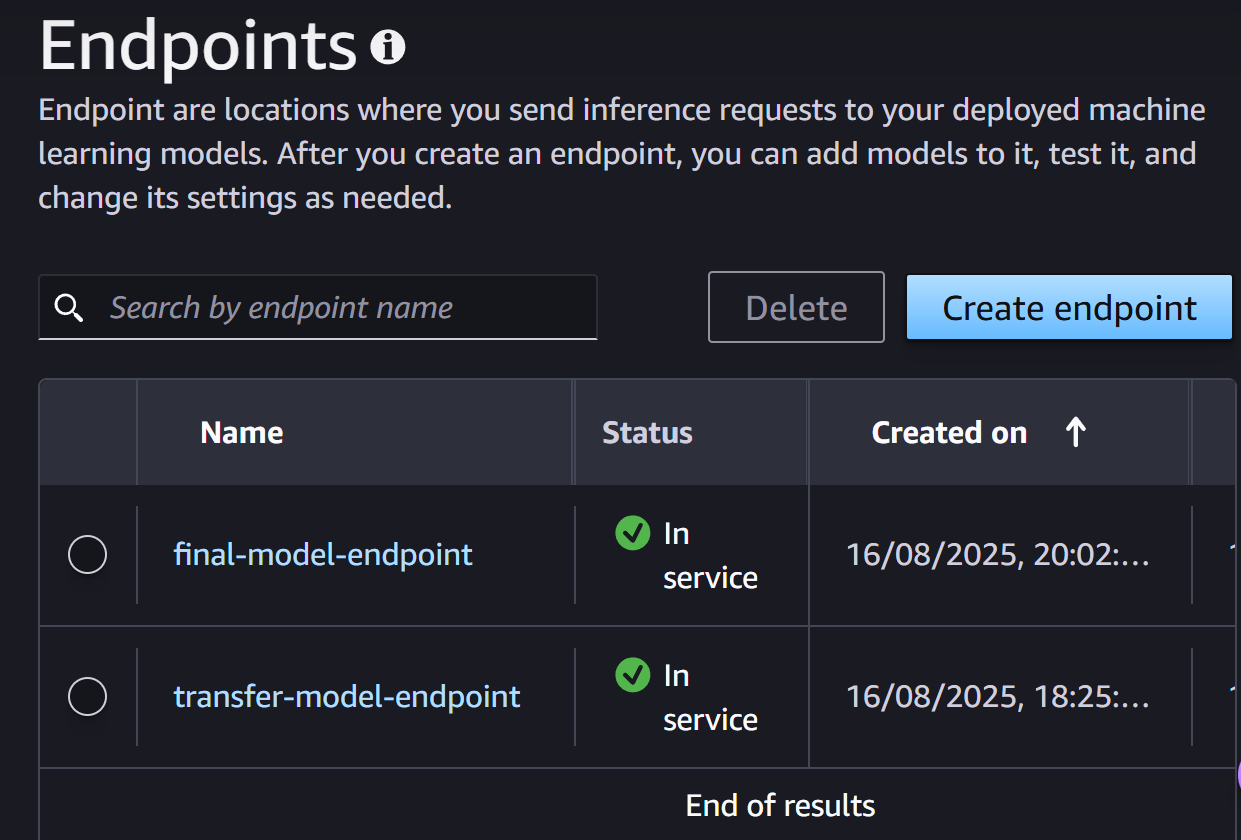
\includegraphics[width=200px]{figures/endpoints_screenshot.png} % Image filename
    \centering
    \caption{Endpoint page screenshot in Sagemaker, as evidence of deployment} % Caption
    \label{fig:endpoint} % Label
\end{figure}

\begin{figure}[h]
    \lstinputlisting[language=Python, caption=Model Deployment and inference code snippet, label=code:deployment_endpoint]{code_chunks/sec_4_example_deployment.py}    
\end{figure}

\newpage

\section{Transfer Learning} \label{sec:transfer_learning}

The list of the possible CNN structures available for use for transfer learning can be seen in \cite{keras_applications}. Of these, EfficientNetV2 was selected as the most suitable architecture due to its demonstrated balance between accuracy and computational efficiency on general image classification tasks. This makes it well-suited for the diverse and varied images present in the aiornot dataset \cite{keras_applications, tan2021efficientnetv2}.

The model used EfficientNetB0, pre-trained on ImageNet, as a feature extractor with its classification head removed and average pooling applied. It was decided to unfreeze the last 10\% of the layers. A dropout layer with rate $p$ was added for regularisation, followed by a final dense layer with sigmoid activation for binary classification. Snippets for the \code{src/transfer_learning.py} file, which was called by the \code{transfer_learning.ipynb} file to train the model can be seen in \cref{code:transfer_learning_code}.

\begin{figure}[h]
    \lstinputlisting[language=Python, caption=Transfer Learning Code Snippet, label=code:transfer_learning_code]{code_chunks/sec_5_transfer_learning.py}
    \label{fig:transfer_learning_code}
\end{figure}

Using an endpoint (using the same deployment strategy as seen previously in \cref{code:deployment_endpoint}), the model was then evaluated on its precision, recall, f1 score, and accuracy. \Cref{fig:endpoint} shows the endpoint configuration in Sagemaker. This allowed for evaluation of the models performance, whilst not being limited by the RAM limitations of the notebook environent in Sagemaker studio. 

Deploying the transfer learning model, again using a sagemaker endpoint allowed a comparison between both models on the holdout set.

\newpage

\section{Model Comparison And Evaluation}

In this section, we compare the performance of the different models trained on the dataset. Evaluation metrics were calculated by invoking the model endpoints on the holdout set, which was not used during training or validation. This ensures that the models' performance is on unseen data, better modelling a general use case.

The endpoints were deployed as real time endpoints, operating on a server and interacting through the user with a HTTP request. While this does mean they can be accessed at any time by any user who has the appropriate permissions, it also means that the network requests are limited to \note{X Mb}, which equates to only 4 500x500 rgb images at a time, making the evaluation process slower. It was for this reason that the holdout set was limited to only 500 images.

\begin{table}[h]
\centering
\caption{Model Comparison}
\begin{tabular}{rcccc}
\toprule
\textbf{Model} & \textbf{Accuracy} & \textbf{Precision} & \textbf{Recall} & \textbf{F1 Score} \\
\midrule
Main Model     & 0.854          & 0.833          & \textbf{0.906} & \textbf{0.868} \\
Transfer Model & \textbf{0.856} & \textbf{0.875} & 0.849 & 0.862 \\
\midrule
$\text{abs}(\text{Difference}) $ & 0.002 & 0.042 & 0.057 & 0.006 \\
\bottomrule
\end{tabular}
\label{tab:model_comparison}
\end{table}

\begin{figure}[h]
    \centering
    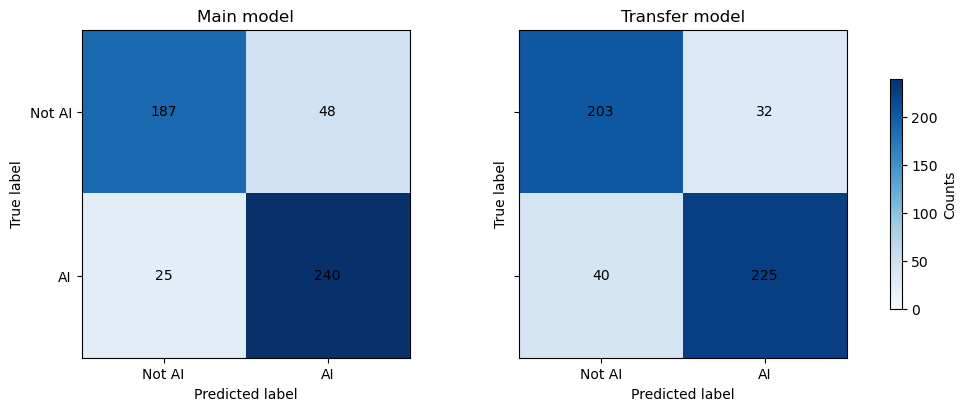
\includegraphics[width=0.9\linewidth]{figures/confusion_matrix.png} % Image filename
    \centering
    \caption{Confusion Matrix of main model and transfer learning model} % Caption
    \label{fig:confusion_matrixes} % Label
\end{figure}

The results of the model evaluation are summarized in \Cref{tab:model_comparison}. The table highlights the key performance indicators for each model. It can be seen that the EfficientNet transfer learning model and the main model have very comparable performance - with the EfficientNet model and main model achieving an accuracy of 85.6\% and 85.4\% respectively - a difference of only 0.2\%. Furthermore the EfficientNet and main model achieved F1 scores of 0.862 and 0.868 respectively, a difference of only 0.006.

Where these models differ is their precision and recall. The EfficientNet model achieved a precision of 87.5\% (4.2\% higher than the main models' 83.3\%.) The main model achieved a recall of 90.6\% (5.7\% higher than the EfficientNet models' 84.9\%.) This means that the EfficientNet model is better at minimising false positive AI detection, whereas the main model is better at detecting AI cases without missing them (i.e. reducing false negatives). 

This is evident in \cref{fig:confusion_matrixes}, where the EfficientNet model has 32 false posiives compared to the main models' 48. Similarly, the main model has only 25 false negatives, compared to the EfficientNet models' 40.

\section{AWS Sagemaker Information and Discussion}

This project was developed using AWS Sagemaker. \Cref{fig:jupyter_lab_space_config} shows the Jupyter lab space configuration used for the project. It can be seen that the smallest option, \code{ml.t3.medium} was used, as model training is done through training jobs, where the compute resources can be chosen to be seperate, allocated to the training job.

\Cref{fig:file_top,fig:file_src} shows the file structure used in the project, run inside the Jupyter lab environment. It can be seen that the model decleration code (\code{src/model_def.py} \& \code{transfer_model.py}) \note{check i say model def everywhyere not just model} and the training code (\code{src/train.py} \& \code{train_transfer.py}) were kept seperate from the main notebooks


\begin{figure}[h]
    \centering
    
\includegraphics[width=0.8\linewidth]{figures/jupyter_lab_space_config.png} % Image filename
    \centering
    \caption{Jupyter lab space configuration screenshot} % Caption
    \label{fig:jupyter_lab_space_config} % Label
\end{figure}

\begin{figure}[htbp]
    \centering
    \begin{minipage}{0.3\textwidth}
        \centering
        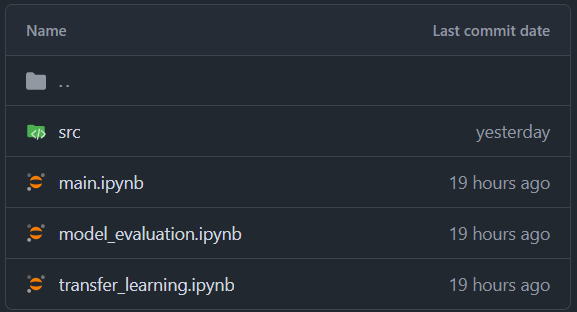
\includegraphics[width=\linewidth]{figures/file_structure_top.png}
        \caption{Top level file structure screenshot}
        \label{fig:file_top}
    \end{minipage}\hfill
    \begin{minipage}{0.3\textwidth}
        \centering
        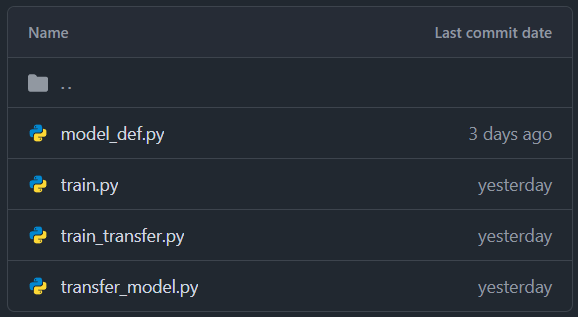
\includegraphics[width=\linewidth]{figures/file_structure_src.png}
        \caption{Files inside the \code{src} directory screenshot}
        \label{fig:file_src}
    \end{minipage}\hfill
    \begin{minipage}{0.35\textwidth}
        \centering
        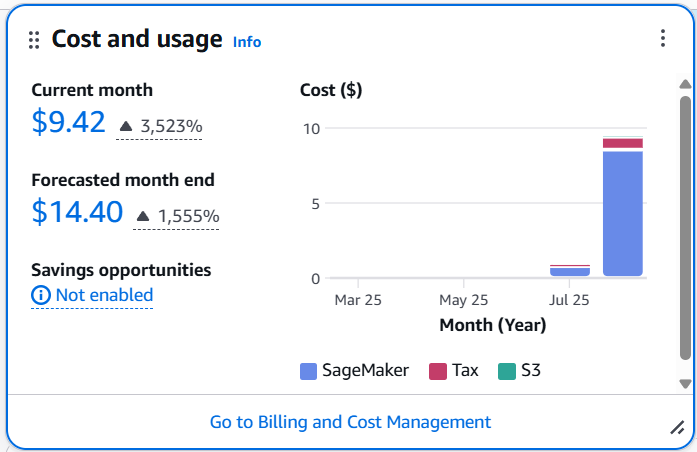
\includegraphics[width=\linewidth]{figures/aws_cost_summary.png} % Image filename
        \caption{Project AWS cost summary screenshot} % Caption
        \label{fig:aws_cost_summary} % Label
    \end{minipage}\hfill
\end{figure}


\Cref{fig:aws_cost_summary} depicts the overall cost summary of the project, which overall was less than \$15. This was achieved due to careful management of resources with a known budget of \$50 leading to selection of smaller instance types (using general purpose ml.c5.2xlarge instances for training and inference rather than larger, more expensive GPU instances). This of course, came at the cost of longer training times, but was deemed acceptable given the budget constraints, and the fact that the workflow would be very easily extensible to a more expensive configuration in a real world deployment scenario.


\note{mention the drawbacks of the deployment here, though have the code chunk (with the creation of the endpoint and the prediction extraction, (and in the appendix have the code snippets for the table and the confusion matrix))}


\note{mention that due to inexperience with sagemaker i ran into memory problems when training the transfer learning model, and therefore had to compromise in having a smaller batch size, and downsampling the images to a resolution of 224x224.}


\newpage

\section{Final Model Discussion and Conclusion}

This report proposed two models to detect if an image is generated using ai - one model developed through hyperparameter tuning, and the other through transfer learning from EfficientNet. The results indicate that both models perform comparably, with slight differences in precision and recall.

The original research objective was to make a tool to distinguish between AI-generated and real images, ultimately as a means to identify the spread of misinformation and other harms in online discourse. Were this model to be deployed as a 'first step' with the intention of more thoughrough investigation, it would be more beneficial to be relaxed on false positives, and minimise false negatives, given the false positives would be vindicated with further analysis or research.

It is for this reason that, assuming this approach, the main model would be the preferred model, as it has a higher recall (90.6\% vs 84.9\%) and therefore is slightly better at detecting AI-generated images without missing them. \note{talk about the paper at the start and that we didnt achieve research level performance, nor the experience to use the dataset they made}


\note{talk about how with more resources, a transfer learning model would be great, as this one was the B0 model, and more beefy models could certainly continue this pattern of good generalisability to this classification task}

\note{mention the limitation of fixed resolutions/aspect ratio of 1:1}

Overall it can be concluded that the models developed in this investigation are effective at distinguising AI-generated images from other images, successfully training and deploying 2 models to make this prediction. 


    \newpage
    \onecolumn
    \section{References}  % This creates a numbered section heading for References
    \bibliographystyle{ieeetran}
    \bibliography{references.bib}

\end{document}